\documentclass{jpconf}

\usepackage{repsty}

\usepackage[utf8]{inputenc}
\usepackage[T1]{fontenc}
\usepackage[english, russian]{babel}

\begin{document}

\title{Статистическая точность при поиске ЭДМ заряженных частиц в накопительных кольцах}
\author{А Е Аксентьев$^{1,2}$, Ю В Сеничев$^2$}
\address{ $^1$ IKP, Forschungszentrum J\"ulich, J\"ulich, Германия}
\address{$^2$ Национальный Исследовательский Ядерный Университет ``МИФИ,'' Москва, Россия}
\ead{a.aksentev@fz-juelich.de}


\begin{abstract}
	На текущий момент, коллаборация “Juelich Electric Dipole moment Investigations” (JEDI), вместе с настоящими экспериментами по поиску ЭДМ на кольце COSY, разрабатывает концептуальный дизайн кольца для поиска дейтронного электрического дипольного момента (дЭДМ). Одной из главных проблем в изучении ЭДМ является прецессия спина в вертикальной плоскости, вызванная неидеальной установкой элементов ускорителя через магнитный дипольный момент (МДМ). Идея разделения ЭДМ и МДМ основана на измерении полной частоты прецессии спина в различающихся процессах и сравнении результата. Высокая точность измерения прецессии спина достигается путём сбора большого количества статистики. Коллаборация JEDI стремится детектировать ЭДМ на уровне $10^{-29}$ e$\cdot$cm, для чего требуется точность оценки частоты $\approx 10^{-9}$ рад/сек. Статистическая точность оценки обусловлена следующими тремя факторами: полное время измерения, определяющее разброс независимой переменной; ошибка измерения; временн\'{a}я модуляция и расстояние между точками выборки. В этой статье мы анализируем взаимосвязь между этими факторами, и оцениваем наилучшую достижимую точность в данных условиях.
\end{abstract}

\section{Модель скорости счёта детектора}
Мы предположим следующую модель для скорости счёта детектора:
\begin{equation}\label{eq:DetCntRt}
	N(t) = N_0(t)\cdot\bkt{1 + P\cdot e^{-\sfrac{t}{\LTd}}\cdot\sin(\omega\cdot t + \phi)},
\end{equation}
где $\LTd$ время декогеренции, и $N_0(t)$ скорость счёта, связанная с неполяризованным сечением взаимодействия.

Поскольку ток пучка может быть выражен как функция времени в виде 
\[
	I(t) \equiv N^b(t)\nu = I_0\cdot e^{\lamb t},
\]
$\lamb$ время жизни пучка, то ожидаемое число частиц, рассеянных в направлении детектора,в течении времени измерения $\dtc$:
\begin{align}
N_0(t) & = p\cdot\int_{-\dtc/2}^{+\dtc/2} I(t+\tau)\td\tau \notag                    \\
& = p\cdot\frac{\nu N_0^b}{\lamb} e^{\lamb t}\cdot \bkt{e^{\lamb\sfrac{\dtc}{2}} - e^{-\lamb\sfrac{\dtc}{2}}} \notag \\
& \approx \underbrace{p\cdot\nu N_0^b e^{\lamb t}}_{\text{rate}~r(t)} \cdot\dtc,
\end{align}
где $p$ вероятность ``полезного'' рассеяния (приблизительно 1\%, согласно Ю.В. Сеничеву, д.ф-м.н., проф. (частная переписка, Декабрь 2016)).

Истинное число детектированных частиц будет распределено в соответствии с распределением Пуассона:
\[
	P_{N_0(t)}(\tilde{N}_0) = \frac{\bkt{r(t)\dtc}^{\tilde{N}_0}}{\tilde{N}_0!}\cdot e^{-r(t)\dtc},
\]
из чего $\SD{\tilde{N}_0}^2(t) = N_0(t)$. %In the limit of large $N_0(t)$, one can use the Gaussian approximation.

Нас интересует математическое ожидание $N_0(t) = \Xpct{\tilde{N}_0(t)}$, и его дисперсия $\SD{N_0}(t)$. Их получают как статистики:
\begin{align*}
	\avg{\tilde{N}_0(t)}[\dtm] &= \frac{1}{\Ncm}\sum_{i=1}^\Ncm \tilde{N}_0(t_i), ~ \Ncm = \dtm/\dtc,
\shortintertext{and} 
	\SD{\tilde{N}_0(t)}[\dtm] &= \frac{1}{\Ncm}\sum_{i=1}^\Ncm \bkt{\tilde{N}_0(t_i) - \avg{\tilde{N}_0(t_i)}[\dtm]}^2.
\end{align*}
($\dtm$ время измерения события, $\dtc$ время измерения поляриметрии.) Будучи суммой рандомных переменных, $N_0(t)$ распределено нормально.

Стандартная ошибка среднего, таким образом, есть % abuse of notation here (SD in place of SE) for aesthetic reasons
\begin{align*}
\SD{N_0}(t) & = \SD{\tilde{N}_0}(t)/\sqrt{\Ncm} = \sqrt{N_0(t)\frac{\dtc}{\dtm}}            \\
& \approx \sqrt{\frac{p\cdot\nu N_0^b}{\dtm}}\cdot\dtc \cdot\exp\bkt{\frac{\lamb}{2}\cdot t}.
\end{align*}
\newcommand{\A}{\frac{1}{\sqrt{p\cdot\nu N_0^b}}}

Относительная ошибка растёт:
\begin{equation}\label{eq:MeasRelErr}
	\frac{\SD{N_0}(t)}{N_0(t)} \approx \frac{A}{\sqrt{\dtm}}\cdot\exp\bkt{-\frac{\lamb}{2}t} = \frac{A}{\sqrt{\dtm}}\cdot\exp\bkt{\frac{t}{2\LTb}},~ A=\A.
\end{equation}

\section{Искомая величина}
\newcommand{\Asym}{\mathcal{A}}
Мероя поляризации пучка является относительная асимметрия скоростей счёта детекторов:~\cite[стр.~17]{Eversmann}
\begin{equation}\label{eq:AsymDef}
	\Asym = \frac{N(\frac\pi2) - N(-\frac\pi2)}{N(\frac\pi2)+N(-\frac\pi2)}.
\end{equation}

В нижеследующей симуляции, данные фитированы функцией
\begin{equation}\label{eq:xFOM}
	\Asym(t) = \Asym(0)\cdot e^{\lamd\cdot t}\cdot\sin\bkt{\omega\cdot t + \phi},
\end{equation}
с тремя параметрами $\Asym(0)$, $\lamd$, и $\phi$. 

Из-за уменьшающегося числа частиц в пучке измерения асимметрии гетероскедастичны. Из~\cite[стр.~18]{Eversmann}, предполагаемая модель гетероскедастичности:
\begin{equation}\label{eq:AsymHtsk}
	\SD{\Asym}^2(t) \approx \frac{1}{2N_0(t)}.
\end{equation}

\section{Условия для максимальной точности}
\DeclareDocumentCommand{\stat}{s}{\IfBooleanTF{#1}{X_{tot}}{\frac{\SD{\meas}^2}{\SE{\hat\omega}^2\cdot \var[w]{t}}}}
\newcommand{\dtnd}{\dt_{zc}}
\newcommand{\SNR}{\text{SNR}}
\newcommand{\deq}{\overset{\triangle}{=}}

Предполагая Гауссово распределение ошибки с нулевым средним и вариацией $\SD{\meas}^2$, максимально-правдоподобная оценка вариации оценки частоты прецессии асимметрии сечения $\Asym$ может быть выражена как
\begin{align*}
\var{\hat\omega} &= \frac{\SD{\meas}^2}{X_{tot}\cdot \var[w]{t}}, 
\shortintertext{with}
X_{tot} &= \sum_{j=1}^{\Nm} x_j = \sum_{s=1}^{\Nnd}\sum_{j=1}^{\Nmnd} x_{js}, \\
\var[w]{t} &= \sum_i w_i \bkt{t_i - \avg{t}[w]}^2,~ \avg{t}[w] = \sum_i w_i t_i, \\
w_i &= \frac{x_i}{\sum_j x_j},~ x_i = (\Asym(0)\exp(\lamd t_i))^2\cos^2(\omega t_i + \phi) = \bkt{\mupp}^2.
\end{align*}

В выражении выше: $X_{tot}$ полная информация Фишера выборки, и $\var[w]{t}$ мера его дисперсии по времени. Можно заметить, что выбирая подходящие моменты для выборки, можно увеличить фактор $X_{tot}$, он пропорционален сумме квадратов производных сигнала по времени. Если частота и фаза уже известны до приелемого уровня точности, дальнейшее улучшение может быть достигнуто путём применения схемы выборки, в которой измерения производятся только во время быстрого изменения сигнала (модуляция сэмплинга). Такое улучшение ограничено только скоростью счёта сигнала детектора.

Оба фактора $\var[w]{t}$ и $X_{tot}$ ограничены в результате декогеренции спина. Мы можем выразить $\sum_{j=1}^{\Nmnd} x_{js} = \Nmnd \cdot x_{0s}$, для некоторого среднего значения $x_{0s}$ в данном узле $s$. $\Nmnd$ --- число измерений асимметрии в узле. Период времени, в течение которого происходят измерения, $\dtnd$, обозначим \emph{время сжатия}. Величина суммы $\sum_{j=1}^{\Nmnd} x_{js}$ падает экспоненциально в результате декогеренции, следовательно $x_{0s} = x_{01}\exp{(\lamd\cdot \frac{(s-1)\cdot\pi}{\omega})}$. Таким образом,
\begin{align}
	X_{tot} & = \Nmnd\cdot x_{01} \cdot \frac{\exp{\bkt{\frac{\lamd\pi}{\omega}\Nnd}}-1}{\exp{\bkt{\frac{\lamd\pi}{\omega}}}-1} 
	\equiv \Nmnd \cdot x_{01}\cdot g(\Nnd); \label{eq:FItot}\\
	x_{01}  & = \frac{1}{\dtnd}\int_{-\dtnd/2}^{+\dtnd/2}\cos^2(\omega\cdot t)\td t = \frac12\cdot \bkt{1 + \frac{\sin\omega\dtnd}{\omega\dtnd}},                                    \label{eq:MeanFIZC}   \\
	\Nmnd   & = \frac{\dtnd}{\dtm}. \label{eq:NumMeasNode}
\end{align}

Уравнение~\eqref{eq:FItot} предоставляет средство для оценки предела длительности эксперимента. В Таблице~\ref{tbl:FItot}, представлены: процент предела полной информации Фишера, время, в течении которого этот предел достигнут (в единицах времени декогеренции), и отношение сигнал/шум к этому времени. Отношение сигнал/шум вычислено в соответствии с:
\begin{equation}\label{eq:TauRatioSNR}
\SNR \deq \frac{\Asym(0)\cdot e^{-\sfrac{t}{\LTd}}}{\SD{\Asym}(t)} 
	\approx \sqrt{2\cdot p\cdot\nu N_0^b\cdot \dtc}\cdot \Asym(0)\cdot \exp\bkt*{-\frac{t}{\LTd}\cdot\bkt{1+\frac12\frac{\LTd}{\LTb}}},
\end{equation}
где, из $\SD{\Asym(0)}/\Asym(0) \approx 3\%$, фактор перед экспонентой равен 33.

\begin{table}[h]
	\caption{Количество информации Фишера (в процентах от доступного предела) содержащееся в сэмпле собранном в течение указанного времени, и соответствующее отношение сигнал/шум.\label{tbl:FItot}}
	
	\centering
	\lineup
	\begin{tabular}{lll}
		\br
		Предел FI (\%) & Длительность ($\times\LTd$) & Сигнал/шум \\
		\mr
		95             & 3.0                         & \00.4      \\
		90                   & 2.3                         & \01.1      \\
		70                   & 1.2                         & \05.5      \\
		50                   & 0.7                         & 11.7       \\
		\br                  &
	\end{tabular}
\end{table}

\section{Симуляция}
Мы симулировали данные из двух детекторов с параметрами собранными в таблице~\ref{tbl:DetCntRtParam} для $T_{tot}=1000$ секунд, собранными равномерно с частотой $f_s = 375$ Гц. Эти величины выбраны по следующей причине: размер пучка за одно заполнение порядка $10^{11}$ частиц; если мы хотим иметь время жизни пучка равное времени декогеренции, мы не можем исчерпать больше 75\% пучка; только 1\% всех рассеяний того сорта, который нам нужен для поляриметрии, так что нам остаётся $\vp{7.5}{8}$ полезных рассеяний. Измерение скорочти счёта детектора $N_0(t)$ с точностью примерно 3\% занимает порядка 2000 событий на детекторе, что ещё убавляет число измерений асимметрии до $\vp{3.75}{5}= f_s\cdot T_{tot}$. Ожидается, что длительность одного заполнения орбиты будет 1000 секунд, поэтому $f_s = 375$ Гц. 

Относительная ошибка скоростей счёта детекторов запечетлена на Рис.~\ref{fig:LRDetErr}; асимметрия сечения, вычисленная в соответствии с уравнением~\eqref{eq:AsymDef}, показана на Рис.~\ref{fig:Asym}.
Эти данные фитируются методом Максимального Правдоподобия нелинейной, гетероскедастичной моделью %\footnote{R package nlreg.~\cite{NLREG}} 
заданной уравнением~\eqref{eq:xFOM}, с функцией дисперсии для весов, заданной уравнением~\eqref{eq:AsymHtsk}. Результаты фитирования собраны в Таблицу~\ref{tbl:FitRes}.
\begin{table}[h]
	\caption{Параметры скорости счёта детекторов.\label{tbl:DetCntRtParam}}
	\centering
	\begin{tabular}{llll}
		\br
		&   Левый   &     Правый     &  \\ \mr
		$\phi$  & $-\pi/2$ &   $+\pi/2$    &   рад   \\
		$\omega$ &  \multicolumn{2}{c}{3}   & рад/сек \\
		$P$    & \multicolumn{2}{c}{0.4}  &  \\
		$\LTd$  & \multicolumn{2}{c}{721}  &   сек   \\
		$\LTb$  & \multicolumn{2}{c}{721}  &   сек   \\
		$N_0(0)$ & \multicolumn{2}{c}{6730} &  \\ \br
	\end{tabular}
\end{table}

\begin{figure}[h]
	\begin{minipage}{.45\textwidth}
		\centering
		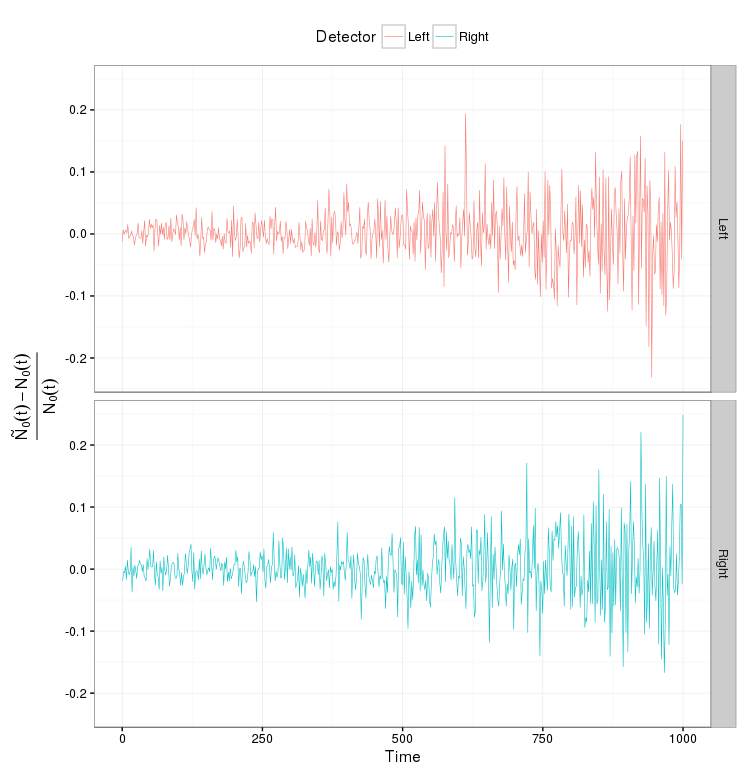
\includegraphics[scale=.4]{img/Final/LR_detector_relErr}
		\caption{Симулированная относительная ошибка измерения скорости счёта для левого и правого детекторов как функция времени.\label{fig:LRDetErr}}
	\end{minipage}\hspace{.5in}
	\begin{minipage}{.45\textwidth}
		\centering
		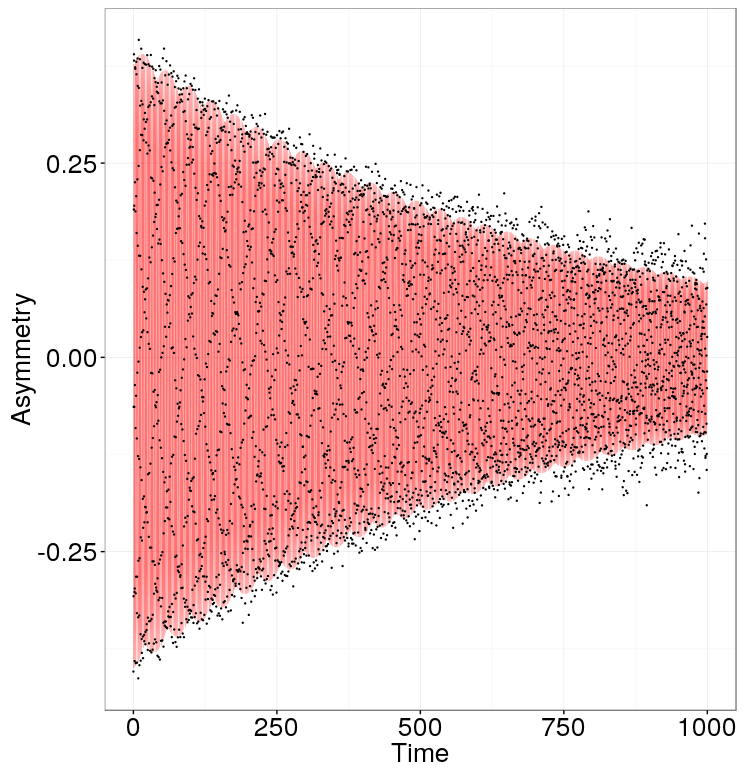
\includegraphics[scale=.4]{img/Final/Asymmetry}
		\caption{Ожидание (красная линия) и измерения выборки (чёрные точки) асимметрии сечения в симуляции.\label{fig:Asym}}
	\end{minipage}
	
\end{figure}

\begin{table}[h]
	\caption{Результаты фитирования асимметрии.\label{tbl:FitRes}}
	\centering
	\lineup
	\begin{tabular}{llll}
		\br
		Параметр  & Оценка & Ошибка              & Единицы    \\ \mr
		$\Asym(0)$ & 0.400  & $\vp{9.03}{-5}$ &  \\
		$\lamd$    & \-0.001   & $\vp{7.86}{-7}$ & 1/сек  \\
		$\omega$   & 3.000  & $\vp{7.55}{-7}$ & рад/сек \\
		$\phi$     & \-1.571   & $\vp{2.25}{-2}$ & рад    \\ \br
	\end{tabular}
\end{table}

\subsection{Улучшение от модуляции}
Если начальная оценка частоты, полученная из равномерно-собранной выборки, имеет стандартную ошибку порядка $\vp{1}{-6}$ рад/сек, симуляции показывают, что стандартная ошибка оценки может быть улучшена до $\approx \vp{5.8}{-7}$ рад/сек.
\\

Этот проект частично поддерживатеся программой Проекта Российской Академической Преуспеваемости ``МИФИ 5/100.''

\section*{Ссылки}

\begin{thebibliography}{9}
%	\bibitem{CountRateStat}
%	\url{http://www.owlnet.rice.edu/~dodds/Files331/stat_notes.pdf}.
	
	\bibitem{Eversmann}
	Eversmann D. Analysis of the Spin Coherence Time at the Cooler Synchrotron COSY [master's thesis on the Internet]. [Aachen (Germany)]: Rheinisch-Westf\"alische Technische Hochschule Aachen (RWTH); 2013 [cited 2017 Feb 28]. Available from: \url{http://wwwo.physik.rwth-aachen.de/fileadmin/user_upload/www_physik/Institute/Inst_3B/Mitarbeiter/Joerg_Pretz/DEMasterarbeit.pdf}
	
	
	
%	\bibitem{NLREG}
%	\url{https://cran.r-project.org/web/packages/nlreg/index.html}
	
\end{thebibliography}

\end{document}